%************************************************
\chapter{Method}\label{ch:method}
%************************************************
\section{Data Preprocessing}

	\subsection{The TIMIT speech corpus}
		TIMIT is a speech corpus that contains phonemically transcribed speech~\citep{garofolo1993darpa}, comprising 6300 sentences, 10 spoken by each of the 630 speakers.
		To include a broad range of dialects all speakers lived in 8 different geographical regions in the United States (as categorized in \cite{labov2008atlas}) during their childhood years.
		Table~\ref{tab:dialects} breaks down the precise composition of the dialect distribution.

		\begin{table}[ht]
		    \myfloatalign
		    \begin{tabularx}{\textwidth}{lrrr} \toprule
		        \tableheadline{Dialect region} & \tableheadline{\#Male}
		        & \tableheadline{\#Female} & \tableheadline{Total} \\ \midrule
		        % Phantoms take care of right-alignment (works iff monospaced digits)
		        1 (New England)   & 31 (63\%) & 18 (27\%) &  49  \phantom{0}(8\%)  \\
		        2 (Northern)      & 71 (70\%) & 31 (30\%) & 102 (16\%) \\
		        3 (North Midland) & 79 (67\%) & 23 (23\%) & 102 (16\%) \\
		        4 (South Midland) & 69 (69\%) & 31 (31\%) & 100 (16\%) \\
		        5 (Southern)      & 62 (63\%) & 36 (37\%) &  98 (16\%) \\
		        6 (New York City) & 30 (65\%) & 16 (35\%) &  46  \phantom{0}(7\%)  \\
		        7 (Western)       & 74 (74\%) & 26 (26\%) & 100 (16\%) \\
		        8                 & 22 (67\%) & 11 (33\%) &  33  \phantom{0}(5\%)  \\
		        \midrule
		        All  & 438 (70\%) & 192 (30\%) & 630 (100\%) \\
		        \bottomrule
		    \end{tabularx}
		    \caption[TIMIT Dialect Regions]{Distibution of speakers' dialect regions and sexes. Speakers of the innominate dialect region 8 relocated often during their childhood.}  \label{tab:dialects}
		\end{table}

		The sentence text can be categorized into 2 \emph{dialect} sentences, 450 \emph{phonetically compact} sentences, and 1890 \emph{phonetically-diverse} sentences.

		The dialect sentences, which are spoken by all speakers, are designed to expose the dialectical variants of the speakers.
		The phonetically compact sentences are designed to include many pairs of phones.
		The phonetically diverse sentences are taken from the Brown Corpus~\citep{kucera1967computational} and the Playwrights Dialog~\citep{hultzsch1964tables} in order to maximize the number of allophones (\ie, different phones used to pronounce the same phoneme).
		Table~\ref{tab:types} lists an overview of the distribution of the number of speakers per sentence type.

		\begin{table}[ht]
		    \myfloatalign
		    \begin{tabularx}{\textwidth}{lrrrr} \toprule
		        \tableheadline{Sentence type} & \tableheadline{\#Sentences}
		        & \tableheadline{\#Speakers} & \tableheadline{Total} \\ \midrule
		        % Phantoms take care of right-alignment (works iff monospaced digits)
		        Dialect & 2    & 630 & 1260\\
		        Compact & 450  & 7   & 3150 \\
		        Diverse & 1890 & 1   & 1890 \\
		        \midrule
		        Total   & 2342 &     & 6300 \\
		        \bottomrule
		    \end{tabularx}
		    \caption[TIMIT Sentence Types]{Distribution of sentence types.}  \label{tab:types}
		\end{table}

		Each of the sentences is encoded in as a waveform signal in \texttt{.wav} format, and is accompanied by a corresponding text file indicating which phones are pronounced in the waveform, and between which pairs of sample points.

	\subsection{Engineering features}

		In this subsection, we describe the preprocessing pipeline as in \cite{fayek2016}, which can be summarized by applying a pre-emphasis filter on the waveforms, then slicing the waveform in short frames, taking their short-term power spectra, computing 26 filterbanks, and finally obtain 12 Mel-Frequency Cepstrum Coefficients (MFCCs).
		We align these MFCCs with the phones found in the TIMIT dataset.
		An example of a waveform signal is given in Figure \ref{fig:signal}.
			\begin{figure}[ht]
				\centering
			    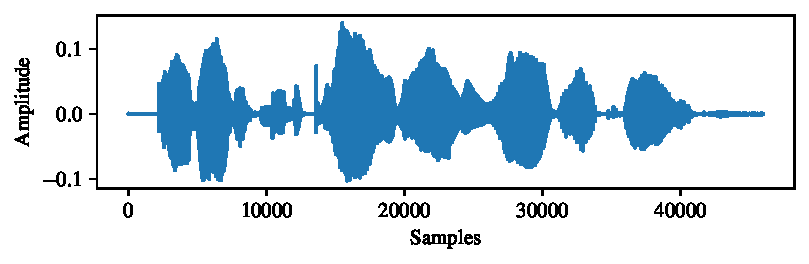
\includegraphics[width=.45\linewidth]{gfx/signal}
			    \label{fig:signal}
			    \caption{A raw waveform signal from the TIMIT dataset.}
			\end{figure}

		\paragraph{Pre-emphasis}

			In speech signals, high frequencies generally have smaller magnitudes than lower frequencies.
			To balance the magnitudes over the range of frequencies in the signal, we apply a pre-emphasis filter $y(t)$ on the waveform signal $x(t)$ defined in Equation \ref{eq:pre_emphasis}.
			\begin{equation}\label{eq:pre_emphasis}
				y(t) = x(t) - 0.97x(t-1)
			\end{equation}
			This procedure yields the additional benefit of improving the signal-to-noise ratio.
			An example of a pre-emphasized signal is given in Figure \ref{fig:signalemph}.
			\begin{figure}[ht]
				\centering
			    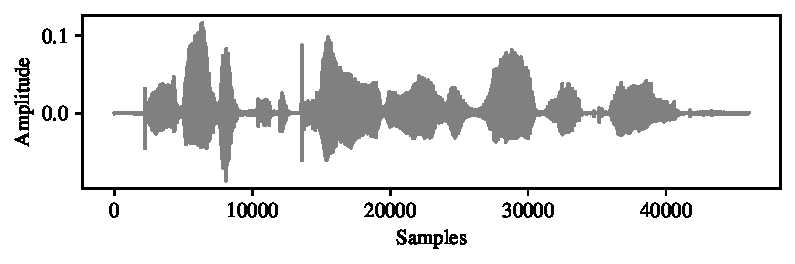
\includegraphics[width=.45\linewidth]{gfx/signalemph}
			    \label{fig:signalemph}
			    \caption[Pre-emphasis]{A signal after the pre-emphasis filter of Equation \ref{eq:pre_emphasis} was applied to it.}
			\end{figure}

		\paragraph{Framing}
			The waveforms, which are sampled at a rate $f_s$ of \SI{16}{\kHz}, cannot be directly used as input to the model, because they are too long---a typical sentence waveform contains in the order of tens of thousands of samples.
			Furthermore, the samples are not very informative, because they represent the sound wave of the uttered sound.
			These sounds are filtered by the shape of the vocal tract, which manifests itself in the envelope of the short time power spectrum of the sound.
			This power spectrum representation describes the power of the frequency components of the signal over a brief interval.
			We assume the frequency components to be stationary over short intervals---in contrast to the full sentence, which carries its meaning because it is non-stationary.
			Therefore, we transform the waveform signals into series of frequency coefficients of short-term power spectra.
			To obtain multiple short-term power spectra over the duration of the waveform, we slice it up into brief overlapping frames.


			Every 160 samples (equivalent to \SI{10}{ms}) of a pre-emphasized signal we take an interval frame of 400 samples (equivalent to \SI{25}{ms}).
			This means that the frames overlap by \SI{25}{ms}.
			The waveform is zero-padded such that the last frame also has 400 samples.
			By this process, we obtain signal frames $x_i(n)$, where $n$ ranges over 1--400, and $i$ ranges over the number of frames in the waveform.

			Then, we apply a Hamming window with the form
			\begin{equation}
				w\left[n\right] = a_0 - a_1\cos\left(\frac{2\pi n}{N-1}\right),
			\end{equation}
			where $N$ is the window length of 400 samples, $0 \leq n < N$, $a_0 = 0.53836$, and $a_1 = 0.46164$.
			A plot of this window is given in Figure \ref{fig:hamming}.
			\begin{figure}[ht]
				\centering
			    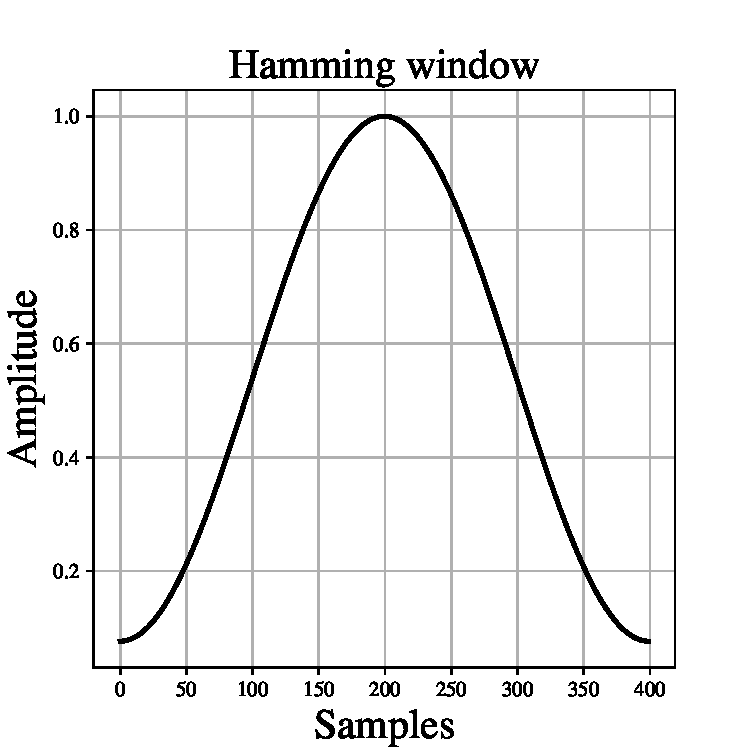
\includegraphics[width=.45\linewidth]{gfx/hamming}
			    \label{fig:hamming}
			    \caption{The magnitudes of the DFT of a frame.}
			\end{figure}
			This window is applied to reduce the spectral leakage, which manifests itself though sidelobes in the power spectra.
			Applying the Hamming window reduces the sidelobes to near-equiripple conditions \citep{SASPWEB2011}.\todo{plot for illustration}.

		\paragraph{Short-term power spectra}

			We obtain the power spectra $P_i$ for each frame by first taking the absolute $K$-point discrete Fourier transform (DFT) of the frame samples $x_i(n)$\todo{don't bother with eqn, just call mathbb(F)}
			\begin{equation}\label{eq:magframes}
				X_k = \left|\sum_{n=0}^{N-1}x_i(n)\cdot e^{-\frac{i2\pi}{N}kn}\right|,
			\end{equation}
			where $K=512$.
			This yields the magnitudes of the DCT of the frames (an example is illustrated in Figure \ref{fig:magframes}).
			\begin{figure}[ht]
				\centering
			    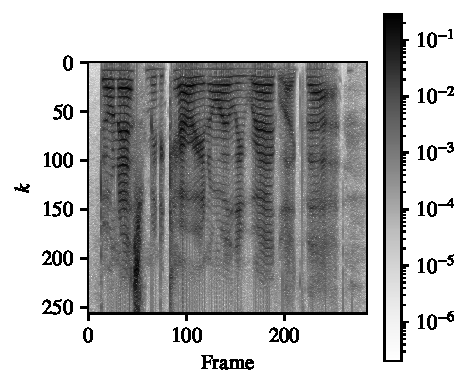
\includegraphics[width=.45\linewidth]{gfx/magframes}
			    \label{fig:magframes}
			    \caption{The magnitudes of the DFT of a frame.}
			\end{figure}

			We obtain the power spectrum using the equation

			\begin{equation}\label{eq:powframes}
				P = \frac{{X_k}^2}{K},
			\end{equation}
			an example of which is shown in Figure \ref{fig:powframes}.

			\begin{figure}[ht]
				\centering
			    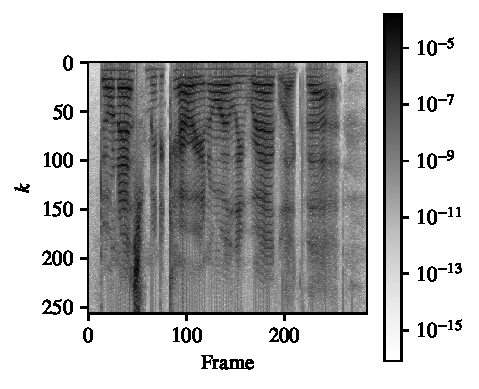
\includegraphics[width=.45\linewidth]{gfx/powframes}
			    \label{fig:powframes}
			    \caption{A power spectrum of a frame.}
			\end{figure}

		\paragraph{Mel filterbank}

			We then transform the short-term power spectra to Mel-spaced filterbanks.
			The Mel scale is a scale of pitches that are perceptually equal in distance \citep{stevens1937scale}.
			This is in contrast to the frequency measurement, in which the human cochlea can better distinguish lower frequencies better than higher ones.
			The aim of converting to the Mel scale is to make every filterbank coefficient feature equally informative, thereby improving the learning performance of the model.

			The Mel-spaced filterbank is a set of 40 triangular filters that we apply to each frame in $P$.

			To compute the Mel-spaced filterbank we choose lower and upper band edges of \SI{0}{\Hz} and $f_s/2 = \SI{8}{\kHz}$, respectively, and convert these to Mels using
			\begin{equation}
				m(f) = 2595\log_{10}\left(1 + \frac{f}{700}\right),
			\end{equation}
			where $f$ is the frequency in $\SI{}{\Hz}$.
			We obtain a lower band edge of 0 Mels and an upper band edge of approximately 2835 Mels.

			We begin obtaining the 40 filterbanks by spacing 42 points $\mathbf{m}$ linearly between these bounds (inclusive).
			Hence, we obtain 42 points spaced exclusively between the bounds.

			Then, we convert each point $m$ back to \SI{}{\Hz} using
			\begin{equation}
				f = 700\left(10^{m/2595}-1\right).
			\end{equation}
			We round each resulting Mel-spaced frequency $f$ to their nearest Fourier transform bin $b$ using
			\begin{equation}
				b = \lfloor(K+1)\mathbf{f}/fs\rfloor
			\end{equation}

			The resulting 40 filterbanks with their corresponding Mels and frequencies are listed in Table \ref{tab:mels}.

			The $i\textsuperscript{th}$ filter in filterbank $H_i$ is a triangular filter that has its lower boundary at $b_{i}$ \SI{}{\Hz}, its peak at $b_{i+1}$ \SI{}{\Hz}, and its upper boundary at $b_{i+2}$ \SI{}{\Hz}.\todo{not sure}
			For other frequencies, they are 0.
			Therefore, the filterbank can be described by
			\begin{equation}
				H_i(k) = \begin{cases}
					0 & k<b_i\\
					\frac{k-b_i}{b_{i+1}-b_i} & b_i\leq k < b_{i+1} \\
					1 & k = b_{i+1} \\
					\frac{b_{i+2} - k}{b_{i+2}-b_{i+1}} & b_{i+1} < k \leq b_{i+2}\\
					0 & b_{i+2} < k
				\end{cases},
			\end{equation}
			where $0 \leq k \leq \frac{K}{2}$.
			These Mel-spaced filters are shown in Figure \ref{fig:filterbank}.
			\begin{figure}[ht]
				\centering
			    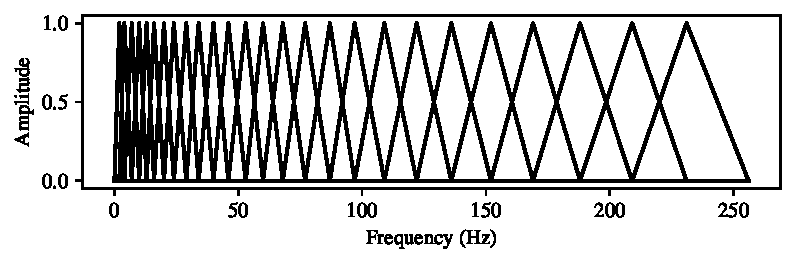
\includegraphics[width=.45\linewidth]{gfx/fbanks}
			    \label{fig:filterbank}
			    \caption{The Mel-spaced filterbanks.}
			\end{figure}

			We obtain a spectrogram $S$ of the frame (see \eg Figure \ref{fig:spectrogram}) after applying the filterbank to the short-term power spectrum.

			\begin{figure}[ht]
				\centering
			    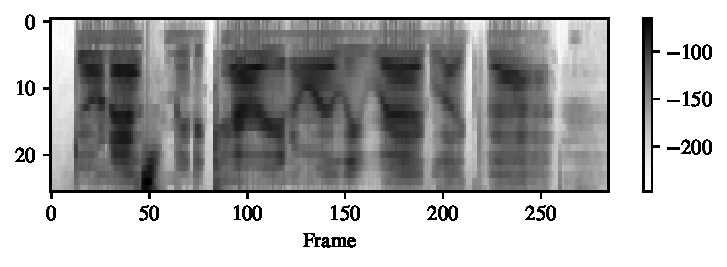
\includegraphics[width=.45\linewidth]{gfx/spectrogram}
			    \label{fig:spectrogram}
			    \caption{An example of a spectrogram.}
			\end{figure}

		\paragraph{Mel-frequency cepstral coefficients}

			We observe that the coefficients in the spectrograms are strongly correlated, which would negatively impact the learning performance of the model \todo{why?}.

			Therefore, we apply the DCT again to decorrelate the coefficients and obtain the power cepstrum $C$ of the speech frame:\todo{do we take absolute?}

			\begin{equation}\label{eq:magframes}
				C(n) = \left|\sum_{n=0}^{N-1}S(n)\cdot e^{-\frac{i2\pi}{N}kn}\right|.
			\end{equation}

			We discard the first coefficient in $C$, because it is the average power of the input signal and therefore carries little meaning.
			We also discard coefficients higher than 13, because they represent only fast changes in the spectrogram and increase the complexity of the input signal while adding increasingly less meaning to it. \todo{source?}
			An example of the remaining MFCC components is shown in Figure \ref{fig:mfccs}.

			\begin{figure}[ht]
				\centering
			    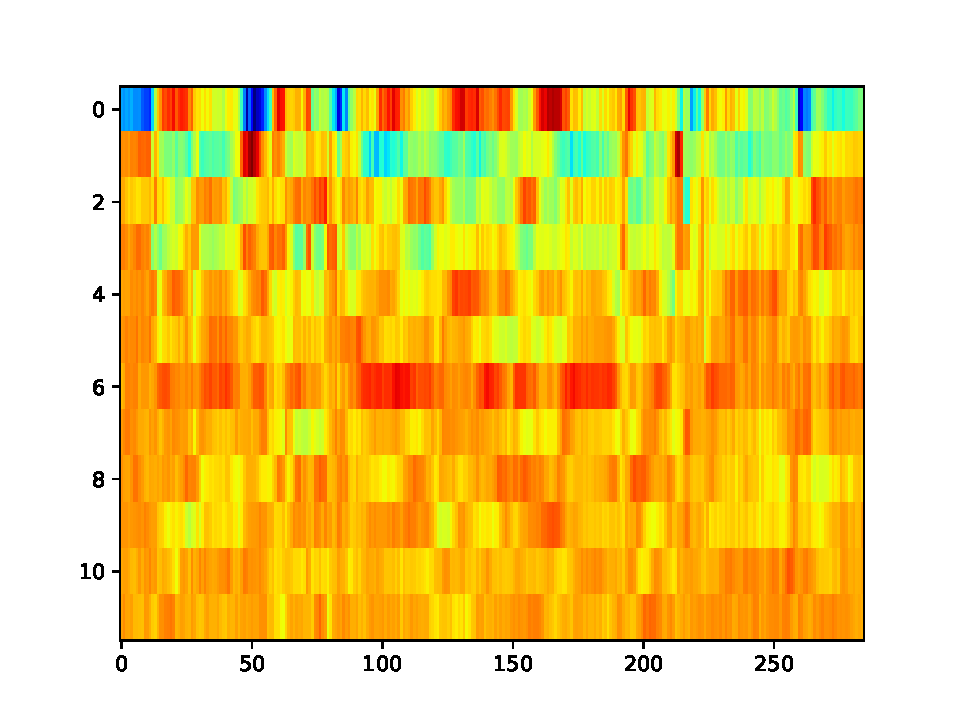
\includegraphics[width=.45\linewidth]{gfx/mfcc}
			    \label{fig:mfccs}
			    \caption{An example of Mel-frequency cepstral coefficients that are given as input to the system.}
			\end{figure}

			Finally, we balance the final MFCCs by centering them around 0 per frame.
			An example of the final MFCCs is given in \ref{fig:source_mfcc_target}.

		\paragraph{Target output}

			The target output of the model is a frame-wise representation of the phones that are uttered in a sentence.
			The TIMIT corpus contains text files indicating in what order phones occur in a sentence, and their starting and ending sample points.

			These phones are discretized into frames such that they align correctly with the MFCCs.
			They are represented in one-hot vector encoding.
			Since the dataset contains 61 different phones, this is also the length of these vectors.

			Figure \ref{fig:source_mfcc_target} illustrates the waveform data and its framewise aligned MFCCs and target output.

			\todo{side-by-side with original text and phonemes, label as fig:source\_mfcc\_target}



		\begin{figure}[ht]
		    \centering
		    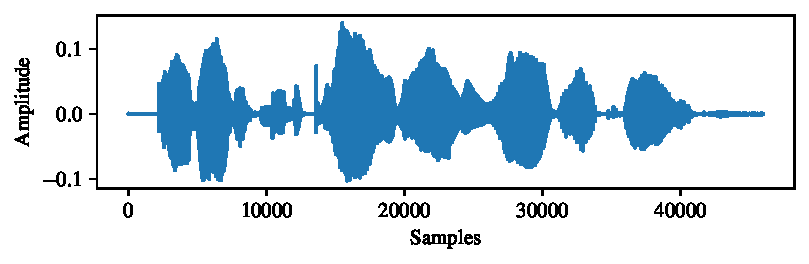
\includegraphics[width=.45\linewidth]{gfx/signal}\\
		    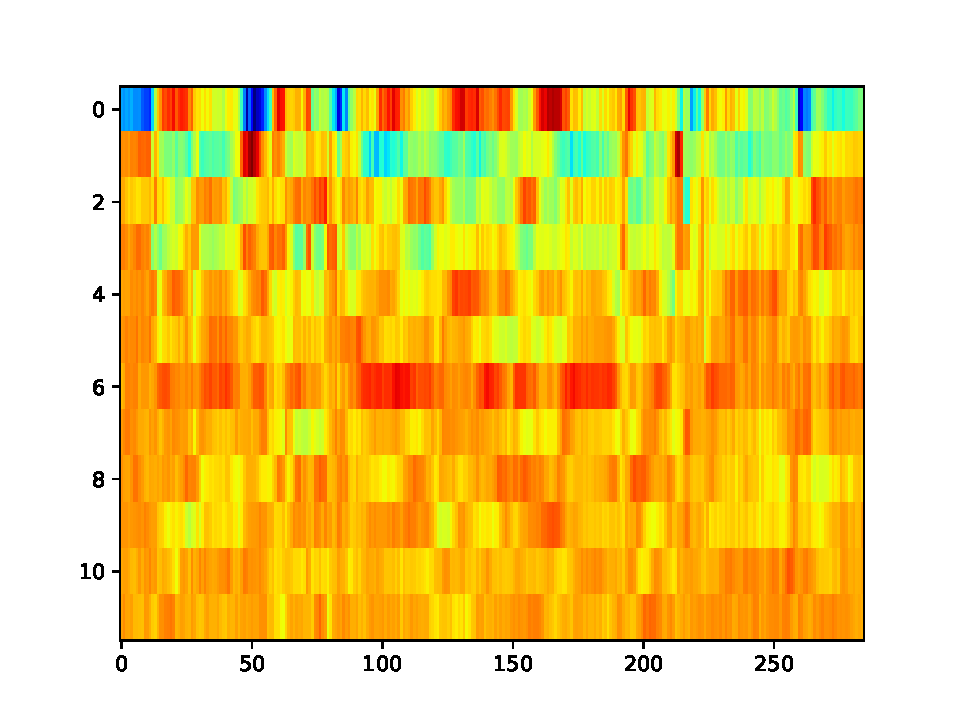
\includegraphics[width=.45\linewidth]{gfx/mfcc}\\
		    % 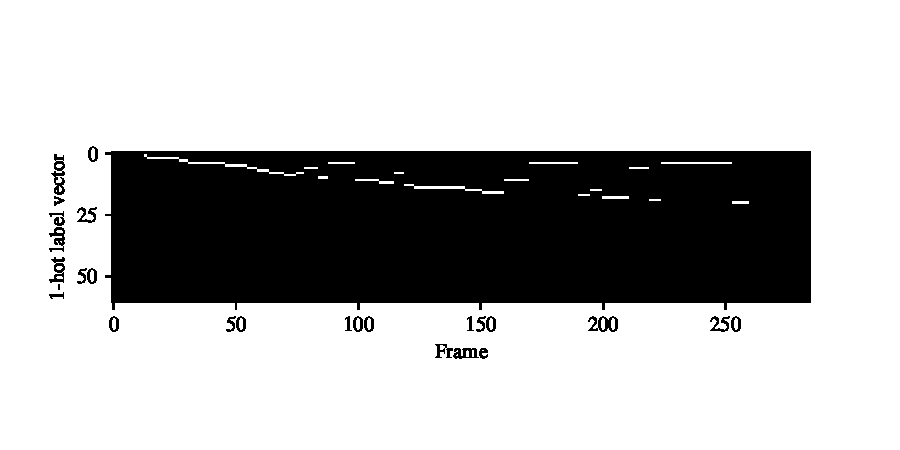
\includegraphics[width=.45\linewidth]{gfx/target}
		    \label{fig:source_mfcc_target}
		    \caption{An alignment of a sample signal with its MFCCs and target phones.}
		\end{figure}


